

\section{On the attaching of $\lambda$-cells}

In this section we will lay the foundations of Morse Theory. Up to this point we have provided the technical apparatus upon which to build the theory; here we will see how Morse functions can serve to relate the homotopy type of a manifold with that of a CW-complex with as many $\lambda$-cells as critical points of index $\lambda$ $f$ has.

\medskip

We begin by introducing some results on vector fields (respecting the vocabulary of \cite{milnor1963}) that will serve us to prove the main results of the section.

\iffalse
Before proving the main results of this section it is worth mentioning what we understand by \textit{Riemannian manifold} and giving a definition of vector field.

\begin{definition}
Let $M$ be a smooth manifold.
We call the \textit{tangent bundle} of $M$ the disjoint union
of the tangent spaces at all the points of $M$, that is,
\[
TM \;=\; \bigsqcup_{p \in M} T_pM.
\]
\end{definition}


\begin{definition}
A \textit{smooth vector field} on a smooth manifold $M$ is a smooth map
\[
X \colon M \to TM,
\]
which we denote $p \mapsto X_p$, and which satisfies that, for every $p \in M$, one has $X_p \in T_pM$.
\end{definition}


\begin{definition}
A \textit{Riemannian manifold} is a pair $(M,\langle\cdot,\cdot\rangle)$ where $M$ is a smooth manifold and for each point $p \in M$, $\langle\cdot,\cdot\rangle_p$ is an inner product (hence bilinear, symmetric and positive definite)
  \[
    \langle\cdot,\cdot\rangle_p \colon T_pM \times T_pM \to \mathbb{R},
  \]
satisfying that for any smooth vector fields $X$ and $Y$, the function
    \[
      p \mapsto \langle X(p), Y(p) \rangle_p
    \]
    is smooth on $M$.
\end{definition}
\fi

\begin{definition}
    Let $M$ be a smooth manifold. We call a \textit{one-parameter group of diffeomorphisms of M} a map $\varphi:\mathbb{R}\times M \to M$ satisfying:
    \begin{enumerate}[label=\roman*)]
        \item For every $t\in \mathbb{R},~~ \varphi_t:M\to M$ defined as $\varphi_t(q)=\varphi(t,q)$, is a diffeomorphism of $M$ onto itself.

        \item For all $t, s\in\mathbb{R}$ one has $\varphi_{t+s}=\varphi_t\circ \varphi_s$.
    \end{enumerate}
\end{definition}

\bigskip

Given a one-parameter group of diffeomorphisms $\varphi$ we define the following vector field on $M$
\begin{equation*}
    X_q(f)=\lim_{h\to 0}\frac{f(\varphi_h(q))-f(q)}{h},
\end{equation*}
where $f$ is a smooth function from $M$ to $\mathbb{R}$, and we say that $X$ generates $\varphi$.

Normally, one refers to the curve $\varphi_\bullet(q): \mathbb{R}\to M,~~ t\mapsto \varphi_t(q)$ as the \textit{flow of X} when the vector field $X$ generating the one-parameter group of diffeomorphisms is known. In any case, we will keep a vocabulary as faithful as possible to the text \cite{milnor1963}.

We will also speak of the \textit{velocity vector} of a differentiable curve $c:\mathbb{R}\to M$, which we define similarly to $X$,
\begin{equation*}
    \frac{dc}{dt}(f)= \lim_{h\to 0}\frac{f(c(t+h))-f(c(t))}{h}\in T_{c(t)}M .
\end{equation*}

\bigskip
\begin{lemma}
\label{unidiff}
    Every vector field on a smooth manifold $M$ that vanishes outside a compact set $K\subset M$ generates a unique one-parameter group of diffeomorphisms of $M$.
\end{lemma}

\begin{proof}
    Let $X$ be a vector field and $\varphi$ a one-parameter group of diffeomorphisms of $M$ generated by $X$. Then we have that, fixing any point $q\in M$, the curve $\varphi_\bullet(q): \mathbb{R}\to M,~~ t\mapsto \varphi_t(q)$ satisfies the differential equation
    \begin{equation*}
        \frac{d\varphi_t}{dt}(q)=X_{\varphi_t(q)}\tag{$\ast$}
    \end{equation*}
    with initial condition $\varphi_0(q)=q$.

    Indeed,
    \begin{align*}
        \frac{d\varphi_t(q)}{dt}(f)=\lim_{h\to 0} \frac{f(\varphi_{t+h}(q))- f(\varphi_t(q))}{h} = \lim_{h\to 0} \frac{f(\varphi_{h}(\varphi_t(q)))- f(\varphi_t(q))}{h} = \lim_{h\to 0} \frac{f(\varphi_{h}(p))- f(p)}{h} = X_p(f),
    \end{align*}

    with $p=\varphi_t(q)$.

    Now, by the Picard--Lindelöf theorem we know that a unique solution exists locally, depending differentiably on the initial condition. That is, for every $ p\in M$ there exist a neighborhood $\mathcal{U}$ of $p$ and $\varepsilon > 0$ such that $(\ast)$ has a unique solution for all $q\in \mathcal{U}$ and $|t|<\varepsilon$.

    Since $K\subset M$ is compact, it can be covered by a finite number of such neighborhoods. Let $\varepsilon_0$ be the smallest of the values defined above and let us set $\varphi_t(q)=q,~~\forall q\notin K$ (hence $X_q=0$ outside $K$). Then $(\ast)$ has a unique solution $\varphi_t(q)$ for $|t|<\varepsilon_0$ and for all $q\in M$, smooth with respect to both variables.

    Let us see that for every suitable $t$ each $\varphi_t$ is a diffeomorphism of $M$ onto itself. For this it suffices to check that $\varphi_{t+s}=\varphi_t\circ \varphi_s$ holds, assuming $|t|,|s|,|t+s|<\varepsilon_0$.

    Let $q\in M$ be fixed and $p=\varphi_s(q)$, then $\varphi_t(p)=\varphi_t(\varphi_s(q))$. We define the curve $\gamma(u)=\varphi_{u+s}(q)$; thus, $\gamma(0)=p$ and

    \begin{equation*}
        \frac{d\gamma}{du}=\frac{d\varphi_{u+s}}{du}(q)=X_{\varphi_{u+s}(q)}=X_{\gamma (u)}.
    \end{equation*}

    Hence $\gamma$ is also a solution of ($\ast$) with initial condition $\gamma(0)=p$.

    However, $\varphi_u(p)$ is also a solution with initial condition $\varphi_0(p)=p$. Hence by uniqueness of solutions
    \begin{equation*}
        \varphi_{u+s}(q)=\gamma(u)=\varphi_u(p)=\varphi_u(\varphi_s(q))=\varphi_u\circ \varphi_s(q),
    \end{equation*}
    whenever $|u|, |u+s|<\varepsilon_0$.

    Lastly, we need to define $\varphi_t$ for all $t\in \mathbb{R}$.

    Let $t\in \mathbb{R}$. Let $k\in \mathbb{Z}$ and $r\in \mathbb{R}$ with $|r|\le \frac{\varepsilon_0}{2}$ be the unique values such that $t=k\frac{\varepsilon_0}{2}+r$. Then we define
    \begin{equation*}
        \varphi_t=\underbrace{\varphi_{\frac{\varepsilon_0}{2}}\circ \dots \circ \varphi_{\frac{\varepsilon_0}{2}}}_{k~times}\circ \varphi_r.
    \end{equation*}

    It is clear that $\varphi:\mathbb{R}\times M\to M$ is a unique diffeomorphism for every $t\in \mathbb{R}$.

\end{proof}

\begin{definition}
    Let $(M,\langle\cdot,\cdot\rangle)$ be a Riemannian manifold and $f:M\to\mathbb{R}$ smooth. The \textit{gradient of f} is defined as the vector field $\nabla f$ satisfying
    \begin{equation*}
        \langle X,\nabla f\rangle = X(f)
    \end{equation*}
    for any other vector field $X$.
\end{definition}
\bigskip
% here I should write something to introduce what follows.

\begin{definition}
    Let $M$ be a smooth manifold and $f:M\to\mathbb{R}$ smooth. We define the \textit{sublevel sets of f} as
    \begin{equation*}
        M^a := f^{-1}(-\infty,a] =\{p\in M: f(p)\le a\}.
    \end{equation*}
\end{definition}

\begin{theorem}
\label{retractodef}
    Let $f:M\to\mathbb{R}$ be smooth on a Riemannian manifold $(M,\langle\cdot,\cdot\rangle)$. Let $a<b$ be real numbers such that $f^{-1}[a,b]$ is compact and contains no critical point of $f$. Then $M^a$ is diffeomorphic to $M^b$. Moreover, $M^a$ is a deformation retract of $M^b$, hence they have the same homotopy type.
\end{theorem}

\begin{proof}
    Let $c:\mathbb{R}\to M$ be a curve with velocity vector $\frac{dc}{dt}$, then
    \begin{equation*}
        \langle \frac{dc}{dt}, \nabla f\rangle = \frac{dc}{dt}(f)=\frac{d(f\circ c)}{dt}.
    \end{equation*}

    We define the smooth map $\rho : M\to \mathbb{R}$ as

    \begin{equation*}
        \rho(p):=
        \begin{cases}
            \frac{1}{\langle \nabla_pf, \nabla_pf\rangle}~~,~p\in f^{-1}[a,b]\\
            0 ~~~~~~~~~~~~~~,p\notin K,
        \end{cases}
    \end{equation*}

    where $K$ is a compact neighborhood of $f^{-1}[a,b]$ % TRANSLATOR: the two cases leave rho unspecified on K \ f^{-1}[a,b]; reproduced as in the original (see IDEAS.md).

    Now, let the vector field be given by $X_q=\rho(q)\nabla_pf$. We have that $X_p$ vanishes outside $K$, hence by Lemma \ref{unidiff} it generates a unique one-parameter group of diffeomorphisms $\varphi_t$ of $M$.

    Let us fix $q\in M$ and consider $f\circ\varphi_{\bullet}(q),~t\mapsto f(\varphi_t(q))$. If $\varphi_t(q)$ is in $f^{-1}[a,b]$ we have
    \begin{align*}
        \frac{df(\varphi_t(q))}{dt} = \left\langle \frac{d\varphi_t(q)}{dt},\nabla f\right\rangle = \langle X, \nabla f\rangle = \langle \rho~ \nabla f, \nabla f\rangle =\\ =\left\langle \frac{1}{\langle \nabla f,\nabla f\rangle}\nabla f,\nabla f\right\rangle=
        \frac{\langle \nabla f,\nabla f\rangle}{\langle \nabla f,\nabla f\rangle}= 1,
    \end{align*}

    so $f(\varphi_t(q))$ is linear with derivative $1$ as long as $f(\varphi_t(q))$ is in $[a,b]$, that is, $f(\varphi_t(q))=f(q)+t$.

    Let us now see that $\varphi_{b-a}$ is a diffeomorphism from $M^a$ to $M^b$.

    Let $q\in M$,
    \begin{equation*}
        \varphi_{b-a}(q)\in M^b \iff(\varphi_{b-a}(q))=f(q)+b-a\le b \iff f(q)-a\le 0 \iff q\in M^a, % TRANSLATOR: "(\varphi_{b-a}(q))" missing "f" reproduced as in the original.
    \end{equation*}
     and in particular it sends the boundary of $M^a$ to the boundary of $M^b$
     \begin{equation*}
         q\in \partial M^a \iff f(q)=a \implies f(\varphi_{b-a}(q))=b \iff b\in \partial M^b. % TRANSLATOR: "b \in \partial M^b" reproduced as in the original; it should be \varphi_{b-a}(q).
     \end{equation*}

     To conclude the proof it remains to check that $M^a$ is indeed a deformation retract of $M^b$. For this we are going to construct a homotopy relative to $M^a$ from the identity of $M^b$ to a retraction of $M^b$ onto $M^a$.

    Let $H(t,q):[0,1]\times M^b\to M^b$ be defined as
    \begin{equation*}
        H(t,q)=
        \begin{cases}
            q,&~f(q)\le a\iff q\in M^a,\\
            \varphi_{t(a-f(q))}(q),&~a\le f(q)\le b.
        \end{cases}
    \end{equation*}

    Then, $H(0,\cdot) = id_{M^b}$ since $\varphi_0(q)=q,~\forall q\in M^b$, and $H(1,\cdot)$ is a retraction of $M^b$ onto $M^a$; let us check it. Let $q\in f^{-1}[a,b]$, we have
    \begin{equation*}
        H(1,q)=f(\varphi_{(a-f(q))}(q))= f(q)+(a-f(q))= a \iff \varphi_{(a-f(q))}(q)\in f^{-1}(a),
    \end{equation*}

    hence $H(1,H(1,\cdot))= id_{M^a}$.

\end{proof}
\begin{remark}
    Note the importance of $f^{-1}[a,b]$ being compact. Let $a=-1/2$ and $b=1/2$ and let our manifold be the sphere $\mathbb{S}^2$ embedded in $\mathbb{R}^3$; it is clear that the function assigning to each point of the sphere its $z$ coordinate is Morse and satisfies that $f^{-1}[a,b]$ is compact since it is closed and the sphere is compact. Now, if we remove from $\mathbb{S}^2$ a point $p$ such that $f(p)$ lies between $f(a)$ and $f(b)$, we have that $f^{-1}[a,b]$ ceases to be compact (as it ceases to be closed and we are in a Hausdorff space) and clearly $M^a$ is not a deformation retract of $M^b$. Indeed, $M^a$ is homeomorphic to a disk and $M^b$ to a punctured disk, which is not simply connected, hence they do not have the same homotopy type. % TRANSLATOR: "between f(a) and f(b)" reproduced as in the original; it should be "between a and b".
\end{remark}
\bigskip

The following theorem is crucial for knowing the CW-complex structure of a manifold. It establishes that the change produced in the homotopy type of the sublevel sets of a Morse function upon crossing a critical point is equivalent to that of attaching a cell of dimension the index of said critical point.

\begin{theorem}
\label{pegadocelula}
     Let $f:M\to\mathbb{R}$ be smooth on a Riemannian manifold $(M,\langle\cdot,\cdot\rangle)$ and $p\in M$ a non-degenerate critical point of $f$ with index $\lambda$. Suppose that $f(p)=c$ and that there exists $\varepsilon>0$ such that $f^{-1}[c-\varepsilon,c+\varepsilon]$ is compact and contains no critical point of $f$ other than $p$. Then, for every sufficiently small $\varepsilon>0$, $M^{c+\varepsilon}_f$ has the homotopy type of $M^{c-\varepsilon}_f$ with a $\lambda$-cell attached.
\end{theorem}

\begin{proof}
    We are going to define a function $F$ that is smaller than $f$ in a neighborhood $\mathcal{U}$ of $p$, with the aim of leaving $p$ outside $F^{-1}[c-\varepsilon, c+\varepsilon]$ and being able to apply Theorem \ref{retractodef} to $F$. In this way, we will have proven that $F^{-1}(-\infty,c-\varepsilon]=M^{c-\varepsilon}_F$ is a deformation retract of $M^{c+\varepsilon}_f$.

    Afterwards, we will prove that $M^{c-\varepsilon}_f$ with a $\lambda$-cell attached is a deformation retract of $M^{c-\varepsilon}_F$ and by the transitivity of this relation we will be done.

    \bigskip
%Preliminaries------------------

    Let $(\mathcal{U}, \phi)$ be a chart of $M$ containing $p$ and $(u^1,\dots , u^n)$ the induced coordinates such that $u^1(p)=\dots=u^{n}(p)=0$. In order to simplify the expressions that follow we define the functions $\xi:\mathcal{U}\to [0,\infty)$ and $\eta:\mathcal{U}\to [0,\infty)$ as
    \begin{gather*}
        \xi(q)=(u^1(q))^2+\dots +(u^{\lambda}(q))^2\\
        \eta(q)=(u^{\lambda +1}(q))^2+\dots +(u^{n}(q))^2
    \end{gather*}
    Applying the Morse Lemma (\ref{lemamorse}) to $f$ we obtain
    \begin{equation*}
        f(q) = c - \xi(q) + \eta(q)
    \end{equation*}
    for each $q\in \mathcal{U}$, where $c=f(p).$

    Let $\varepsilon>0$ be small enough so that:
    \begin{enumerate}[label=\roman*)]
        \item $f^{-1}[c-\varepsilon,c+\varepsilon]$ is compact and contains no critical point of $f$ other than $p$.
        \item $\phi(\mathcal{U})\subset \mathbb{R}^n$ contains the closed ball
        \begin{equation*}
            \phi\left(\overline{B(0, \sqrt{2\varepsilon})}\right)= \{q\in \mathcal{U}: \xi(q)+\eta(q)\le 2\varepsilon\}
        \end{equation*}
    \end{enumerate}

%Construction of F----------------
    Let us construct $F:M\to \mathbb{R}$. Let $\mu:\mathbb{R}\to\mathbb{R}$ be a smooth map satisfying the following
    \begin{equation*}
        \begin{cases}
        \mu(0)>\varepsilon\\[3pt]
        \mu(r)=0, ~~r\ge 2\varepsilon\\[3pt]
        -1<\mu'(r)\le 0, ~~\forall r\in \mathbb{R},
        \end{cases}
    \end{equation*}
    then we define $F$ as
    \vspace{1em}
    \begin{equation*}
        F(q)=
        \begin{cases}
        f(q),&~~q\notin \mathcal{U},\\
        f(q)- \mu(\xi(q)+2\eta(q)),&~~q\in \mathcal{U}.
        \end{cases}
    \end{equation*}

    It is clear that $F$ is well defined since $\mu$ vanishes on $\partial\mathcal{U}$. Moreover, it is smooth since in a neighborhood of $\partial\mathcal{U}$ one has that $\mu'$ is identically $0$, hence both approaching from inside $\mathcal{U}$ and from outside $d_qF=d_qf$.

    \bigskip

%First retraction-------------------------------

    Now that we have $F$ we must check that we are within the hypotheses of Theorem \ref{retractodef}. Let us see first that $M_F^{c+\varepsilon}=M_f^{c+\varepsilon}$, then that $F$ and $f$ possess the same critical points and that $F^{-1}[c-\varepsilon,c+\varepsilon]$ contains no critical point.

    Indeed, $\mu(\xi(q)+2\eta(q))=0$ for every $q\in M$ such that $\xi(q)+2\eta(q)\ge 2\varepsilon$, hence outside the ellipsoid $E=\{q\in M:\xi(q)+2\eta(q)\le 2\varepsilon\}$ we have that $F=f$.

    \medskip

    We know that $E\subset M_f^{c+\varepsilon}$ and by
    \begin{equation*}
        F(q)<f(q)=c-\xi(q)+\eta(q)\le c+\frac{1}{2}\xi(q)+\eta\le c + \varepsilon, ~\forall q\in E, % TRANSLATOR: "\eta" missing its argument (q) reproduced as in the original.
    \end{equation*}

    we have that $E\subset M_F^{c+\varepsilon}$. Seeing that it is the only region on which they differ, we conclude that $M_F^{c+\varepsilon}=M_f^{c+\varepsilon}$.

    \medskip

    Now let us see that their critical points coincide. We observe that on $\mathcal{U}$ the following hold
    \begin{align*}
        \frac{\partial F}{\partial \xi}&=-1-\mu'(\xi + 2\eta)<0 ~\text{ and}\\
        \frac{\partial F}{\partial \eta}&=1-2\mu'(\xi+2\eta)\ge 1.
    \end{align*}
    The critical points of $F$ will be those annihilating its partial derivatives
    \begin{align*}
        \frac{\partial F}{\partial x_i}=\frac{\partial F}{\partial \xi}\frac{\partial \xi}{\partial x_i} + \frac{\partial F}{\partial \eta}\frac{\partial \eta}{\partial x_i},
    \end{align*}

    but the only point simultaneously satisfying $\frac{\partial \xi}{\partial x_i}=0$ and $\frac{\partial \eta}{\partial x_i}=0$ is $p$, since otherwise $f$ would have more critical points in $\mathcal{U}$. Hence, as they coincide outside $\mathcal{U}$, we have that $F$ and $f$ have the same critical points.

    \medskip

    Let us see that $F^{-1}[c-\varepsilon,c+\varepsilon]=M^{c+\varepsilon}_F\setminus M^{c-\varepsilon}_F$ is compact and contains no critical point. It is clear that $M^{c-\varepsilon}_f\subset M^{c-\varepsilon}_F$ since $F$ and $f$ coincide except on the neighborhood of $p$ on which $F\le f$, thus
    \begin{equation*}
        M^{c+\varepsilon}_F=M^{c+\varepsilon}_f\implies M^{c+\varepsilon}_F\setminus M^{c-\varepsilon}_F \subset M^{c+\varepsilon}_f\setminus M^{c-\varepsilon}_f=f^{-1}[c-\varepsilon,c+\varepsilon],
    \end{equation*}
    whereby $F^{-1}[c-\varepsilon,c+\varepsilon]$ is compact. On the other hand,
    \begin{equation*}
        F(p)=c-\mu(0)<c-\varepsilon,
    \end{equation*}

    hence $p\notin F^{-1}[c-\varepsilon,c+\varepsilon]$.

    \medskip

    In this way, we find ourselves within the hypotheses of Theorem \ref{retractodef} for $F$, which proves that $M^{c-\varepsilon}_F$ is a deformation retract of $M^{c+\varepsilon}_F=M^{c+\varepsilon}_f$.

    \bigskip

%Second retraction------------------

    Let $e^{\lambda}=\{q\in \mathcal{U}: \xi(q)\le \varepsilon,~\eta(q)=0 \}\subset \mathcal{U}$ be a $\lambda$-cell. First of all, let us see that
    \begin{equation*}
        \partial e^{\lambda}=\{q\in \mathcal{U}: \xi(q)= \varepsilon,~~\eta(q)=0 \}=M^{c-\varepsilon}_f\cap e^{\lambda}.
    \end{equation*}
    Indeed:
    \begin{quote}
    $\left( \subseteq \right) ~~\text{For all }~ q\in \partial e^{\lambda},~f(q)=c-\varepsilon \implies q\in M^{c-\varepsilon}_f$.

    $\left( \supseteq \right) ~~\text{For all }~ q\in M^{c-\varepsilon}_f\cap e^{\lambda}$, we have $\xi(q)\le\varepsilon,~\eta(q)=0 \text{ and } f(q)\le -\varepsilon$, then since % TRANSLATOR: "f(q) <= -epsilon" reproduced as in the original; it should be c-epsilon.
    \begin{equation*}
        f(q)=c-\xi(q)\le c-\varepsilon\iff \xi(q)\ge \varepsilon
    \end{equation*}
    \quad \quad necessarily $\xi(q)=\varepsilon$, hence $q\in \partial e^{\lambda}$.
    \end{quote}
    \bigskip

    Figure \ref{fig:diagrama1} shows the sublevel sets of $f$ and the $\lambda$-cell. The axes correspond to the planes $u^{\lambda+1}=\dots=u^n=0$ and $u^{1}=\dots=u^{\lambda}=0$. The circle represents the boundary of the ball of radius $\sqrt{2\varepsilon}$ and center $p$. The darkest region corresponds to $M^{c-\varepsilon}_f$, the region with large dots is $f^{-1}[c-\varepsilon,c]$ and, finally, the region with the smallest dots is $f^{-1}[c,c+\varepsilon]$.

    \begin{figure}[H]
        \centering
        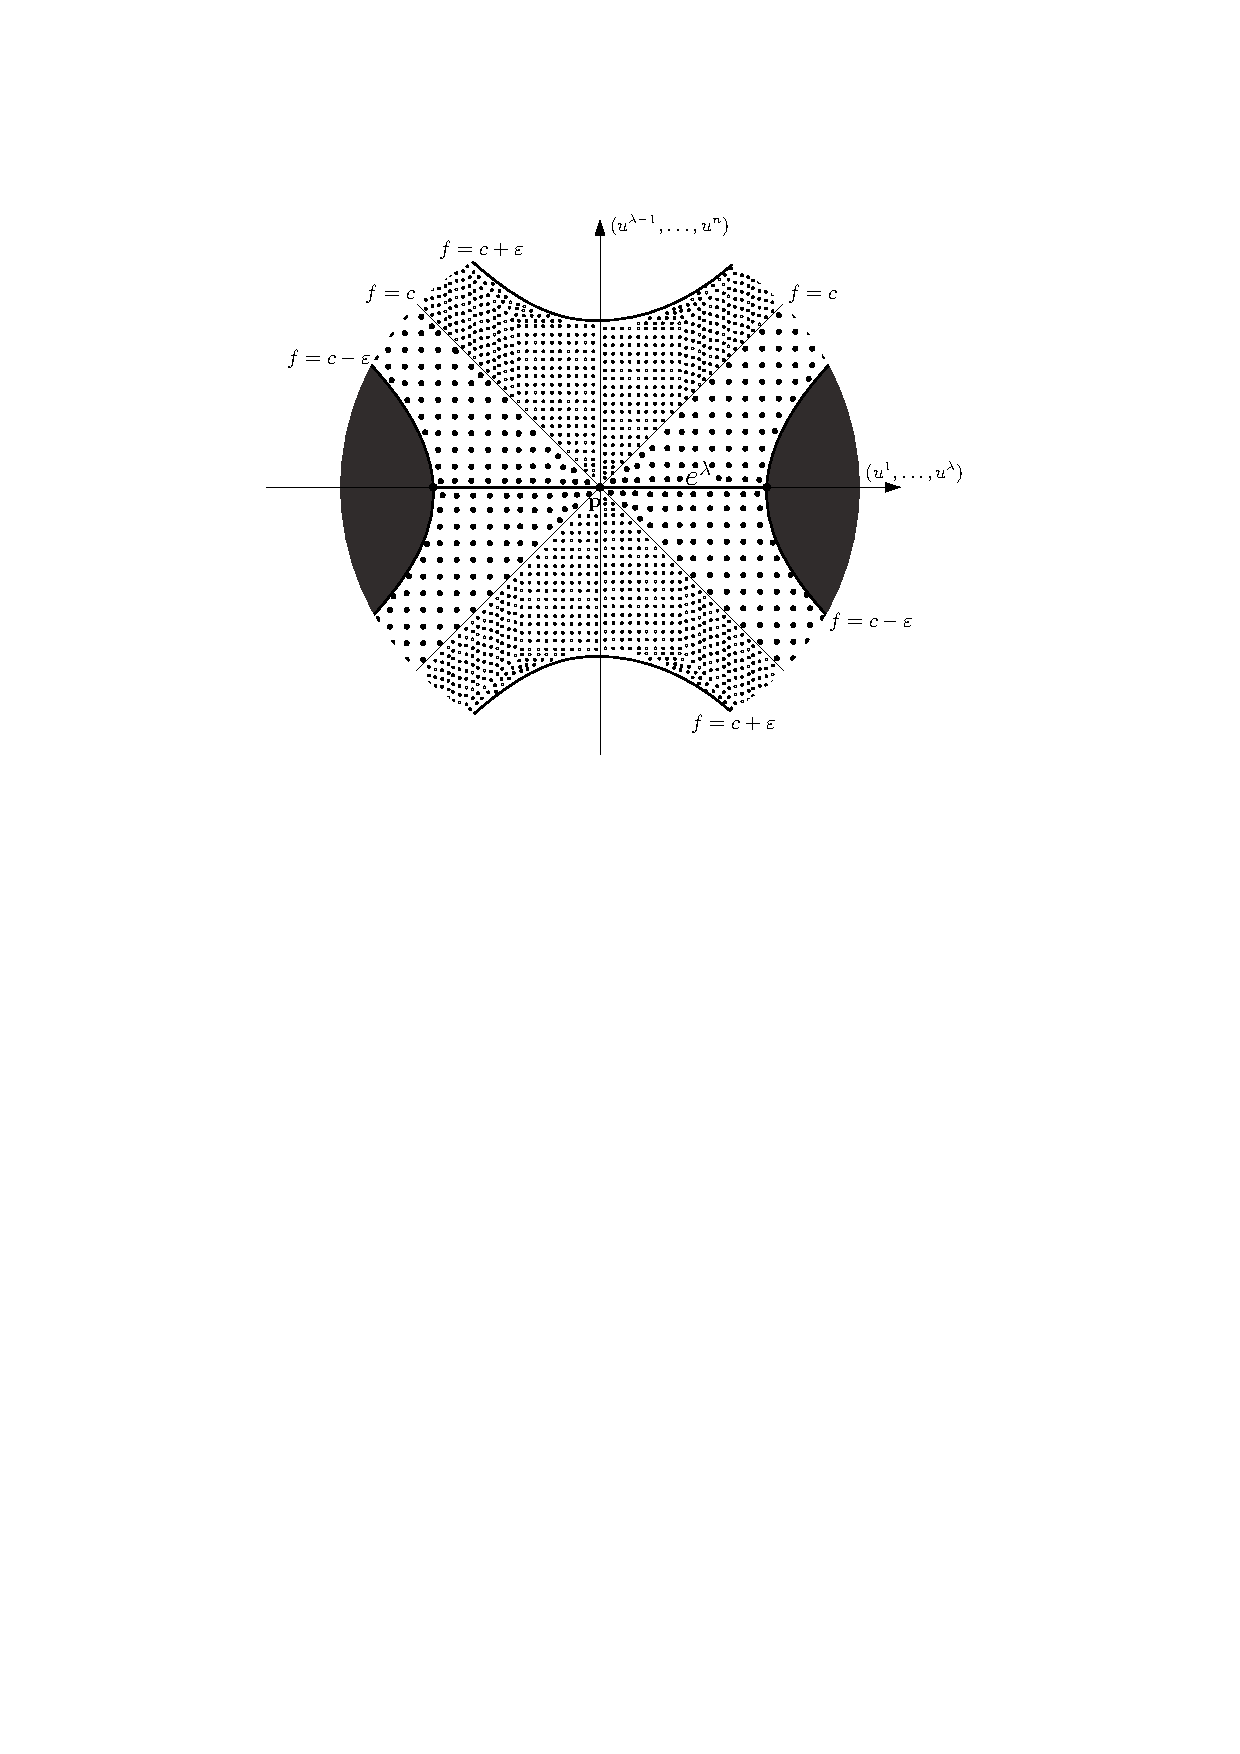
\includegraphics[width=0.8\textwidth]{imagenes/diagrama1_def.pdf}
        \caption{Schematic representation of the neighborhood of the critical point $p$ with respect to $f$.}
        \label{fig:diagrama1}
    \end{figure}




    For the rest of the proof it will turn out convenient to introduce the notion of \textit{handle}. We will understand $M_F^{c-\varepsilon}$ as $M_f^{c-\varepsilon}\cup H$ where $H=\overline{M_F^{c-\varepsilon}\setminus M_f^{c-\varepsilon}}$ is the handle we speak of, denoted this way by virtue of its English name \textit{handle}. % TRANSLATOR: the Spanish original introduces "asa" and notes its English name; the aside is kept for faithfulness.

    \medskip

    We observe that $e^{\lambda}$ is contained in $H$. Indeed, $F$ attains its maximum on $\mathcal{U}$ when $\mu(\xi+2\eta)$ attains its minimum, and the latter attains it when $\xi$ and $\eta$ vanish, that is, only at $p$, thus % TRANSLATOR: max/min justification garbled in the original (F = f - mu); the displayed inequalities below are what carry the argument (see IDEAS.md).
    \begin{equation*}
        F(q)\le F(p)<c-\varepsilon ~\text{ and }~f(q)=c-\xi(q)\ge c-\varepsilon,~\forall q\in e^{\lambda},
    \end{equation*}
    hence $q\in e^{\lambda}$ which implies that $q$ is in $H$.

    \medskip


    Now we want to prove that $M^{c-\varepsilon}_f\cup e^{\lambda}$ is a deformation retract of $M^{c-\varepsilon}_F = M_f^{c-\varepsilon}\cup H$. For this we are going to construct a homotopy relative to $M^{c-\varepsilon}_f\cup e^{\lambda}$ from the identity to a retraction onto $M^{c-\varepsilon}_f\cup e^{\lambda}$, as in the proof of Theorem \ref{retractodef}.

    Figure \ref{fig:diagrama_asa} shows the neighborhood of $p$ from this perspective. The dark zone represents $M_f^{c-\varepsilon}$, the dotted zone corresponds to $F^{-1}[c-\varepsilon,c+\varepsilon]=M^{c+\varepsilon}_F\setminus M^{c-\varepsilon}_F$ and the zone with arrows is $H$, the handle. Besides identifying $H$, the arrows illustrate the deformation we will carry out in the next and final step of the proof.


    \begin{figure}[H]
        \centering
        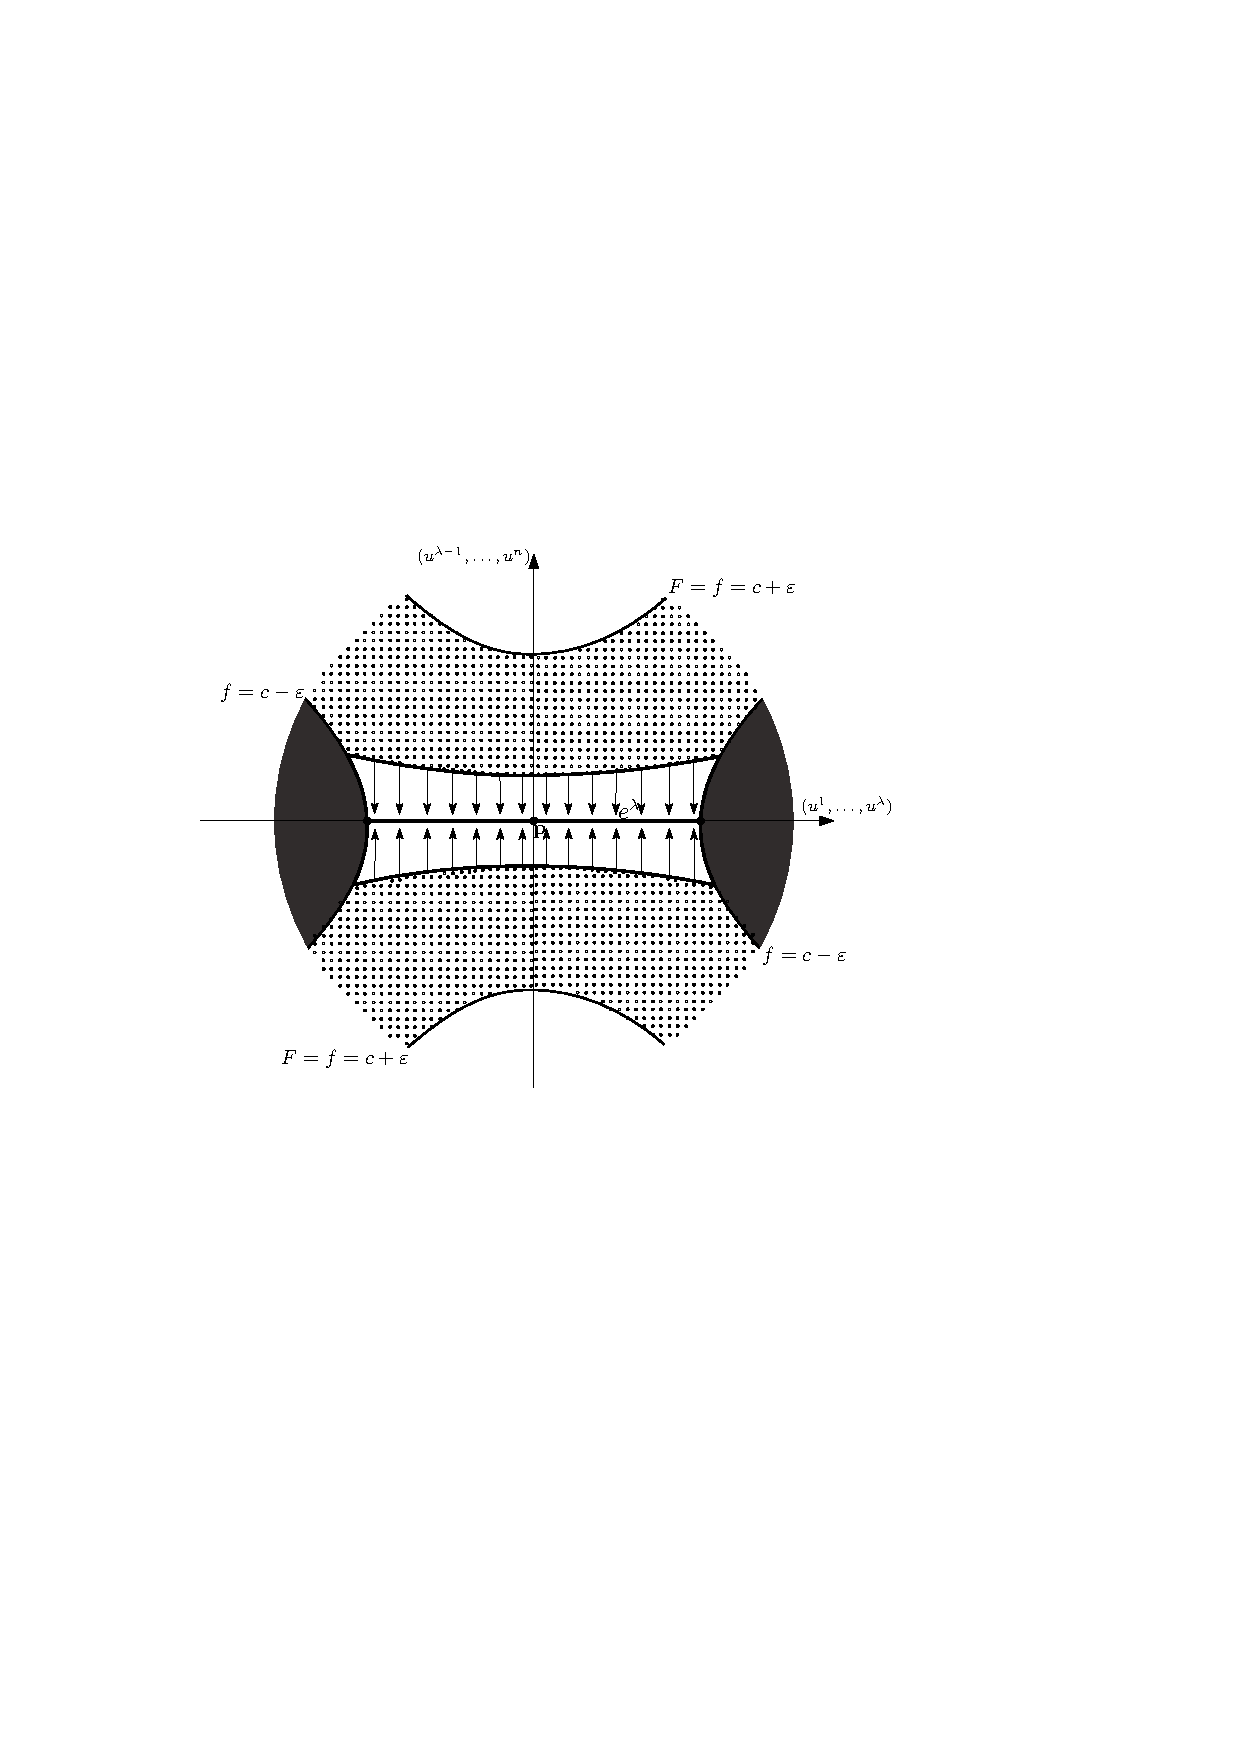
\includegraphics[width=0.8\textwidth]{imagenes/diagrama2_asa.pdf}
        \caption{Schematic representation of the neighborhood of the critical point $p$ with respect to $F$ and with the handle.}
        \label{fig:diagrama_asa}
    \end{figure}

    \bigskip

    Let $\Psi:[0,1]\times M_f^{c-\varepsilon}\cup H\to M_f^{c-\varepsilon}\cup H$; we define $\Psi$ as the identity outside $\mathcal{U}$. On $\mathcal{U}$ we must distinguish three regions.

    Figure \ref{fig:diagrama_asa_regiones} shows schematically the regions into which $\mathcal{U}$ is divided near the handle. The zone with black-tipped arrows represents the part of region $1$ lying inside the handle. The zone with the small hollow-tipped arrows coincides with the part of region $2$ lying inside the handle. The dark zone is region $3$. Likewise, the arrows illustrate which part of the handle we want to deform and onto what. Note that in region $3$ nothing needs to be deformed.
    \medskip

    \textbf{Region 1:}\quad $R_1=\{q\in\mathcal{U}:\xi(q)\le \varepsilon\}$.

    In this region what we want is to take the points to $e^{\lambda}$.

    We define $\Psi(t,q)=\Psi(t,(u_1(q),\dots,u_n(q))=(u_1(q),\dots,u_{\lambda}(q),tu_{\lambda+1}(q),\dots,tu_n(q))$.
    \bigskip

    It is clear that it is relative to $M^{c-\varepsilon}_f\cup e^{\lambda}$ ($R_1\cap M^{c-\varepsilon}_f=\varnothing$ and it does not touch the points of $e^{\lambda}$) and that $\Psi(1,\cdot)$ is the identity. Moreover,
    \begin{equation*}
        \forall q\in R_1, ~\Psi(0, q)\in e^{\lambda} ~\text{ and }~ \Psi(0,\Psi(0,q))=\Psi(0,q).
    \end{equation*}

    Likewise, since $\frac{\partial F}{\partial \eta}>0$ (that is, $F$ grows in the direction of $\eta$) we have that $F(\Psi(t,q))\le F(q)$ for all $t\in [0,1]$ and all $q\in R_1$. Hence $\Psi$ takes $M_f^{c-\varepsilon}\cup H$ into itself.
    \bigskip

    \textbf{Region 2:}\quad $R_2=\{q\in \mathcal{U}:~ \varepsilon\le \xi(q)\le \eta(q)+\varepsilon\}$.


    Here what we seek is to take the points of $R_2$ to the boundary of $M_f^{c-\varepsilon}$.

    We define $\Psi(t,q)=\Psi(t,(u_1(q),\dots,u_n(q))=(u_1(q),\dots,u_{\lambda}(q),s_t(q) u_{\lambda+1}(q),\dots,s_t(q) u_n(q))$, where
    \begin{equation*}
        s_t(q)=t + (1-t)\left(\frac{\xi(q)-\varepsilon}{\eta}\right)^{1/2} \in ~[0,1]
    \end{equation*}

    Just as on $R_1$ it is clear that it is relative to $M_f^{c-\varepsilon}\cup e^{\lambda}$, that $D(1,\cdot)$ is again the identity and that $\Psi(0,\cdot)$ is a retraction onto the boundary of $M_f^{c-\varepsilon}$. The latter follows from the fact that on the boundary of $M_f^{c-\varepsilon}$ one has $-\xi +\eta = \varepsilon$, hence $s_0(q)=1$. % TRANSLATOR: "D(1,.)" reproduced as in the original; it should be \Psi(1,.). Also "-xi+eta=epsilon" describes f=c-epsilon, i.e. xi-eta=epsilon; sign slip reproduced.

    It remains to see that $s_t$ is continuous as $\xi \to \varepsilon$ and $\eta \to 0$. Rearranging the inequality defining $R_2$ we have $0\le\xi-\varepsilon\le\eta$, which means that as $\eta$ tends to zero, $\xi$ must tend to $\varepsilon$ faster. Thus,
    \begin{equation*}
        0\le \lim_{\xi \to \varepsilon, \eta\to 0} \frac{\xi - \varepsilon}{\eta} \le 1
    \end{equation*}
    and in particular, we have that $\lim_{\xi \to \varepsilon, \eta\to 0} \frac{\xi - \varepsilon}{\eta}=0$ necessarily. We conclude then that $s_t$ generates no problems in the continuity of $\Psi$ near the points with $\eta(q)=0$. % TRANSLATOR: the limit claim is a non sequitur in the original (the limit need not exist, nor be 0); reproduced faithfully (see IDEAS.md).
    \bigskip

    \textbf{Region 3:}\quad $R_3=\{q\in \mathcal{U}:~ \eta(q) + \varepsilon \le \xi(q)\}$


    $R_3$ coincides with $M_f^{c-\varepsilon}$, hence it suffices to take $\Psi(t,q)= Id_{M_f^{c-\varepsilon}}$.
    \bigskip

    \begin{figure}[H]
        \centering
        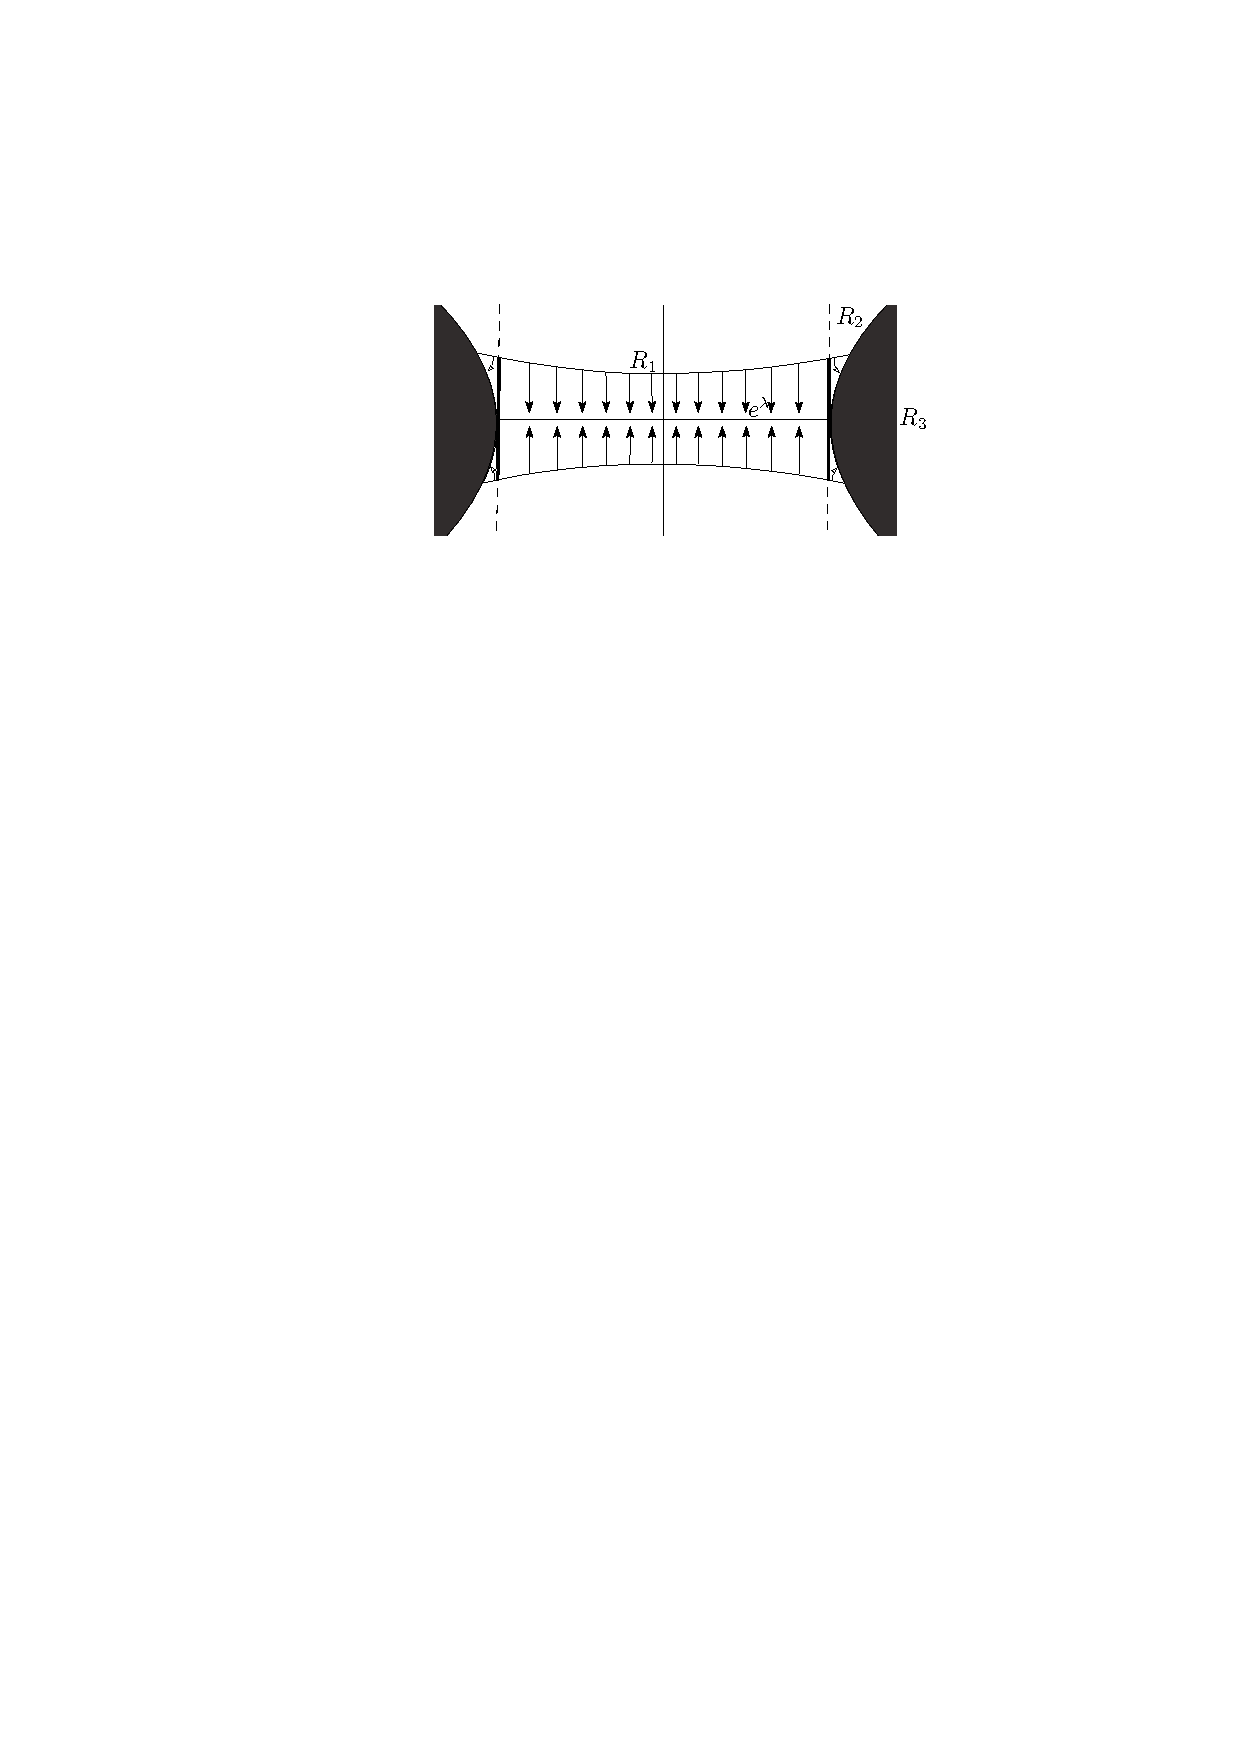
\includegraphics[width=0.7\textwidth]{imagenes/diagrama_asa_regiones.pdf}
        \caption{Schematic representation of the regions into which the handle is divided.}
        \label{fig:diagrama_asa_regiones}
    \end{figure}


    The three regions completely cover $\mathcal{U}$. This concludes the proof that $M^{c-\varepsilon}_f\cup e^{\lambda}$ is a deformation retract of $M^{c-\varepsilon}_F = M_f^{c-\varepsilon}\cup H$ and with it the proof of the theorem.

\end{proof}
\begin{remark}
\label{obs_incluso_con_c_critico}
    \hfill
    \begin{enumerate}[label=(\roman*)]
        \item By modifying the proof a little it is possible to prove that $M^c_f$ is also a deformation retract of $M^{c+\varepsilon}_f$. In fact, $M^c_f$ is a deformation retract of $M_F^c$, which is in turn a deformation retract of $M^{c+\varepsilon}_f$; this, together with the theorem, makes it clear that $M^{c-\varepsilon}_f\cup e^{\lambda}$ is a deformation retract of $M^c_f$.
        \item Furthermore, as a corollary of this proof it follows that $M^{c+\varepsilon}_f$ is not only homotopy equivalent but homeomorphic to $M^{c-\varepsilon}$ with a $\lambda$-handle $D^\lambda \times D^{n-\lambda}$ attached. In case $M$ is compact, doing this at each critical point gives rise to a decomposition of $M$ into successive attachings of handles known as a ``handlebody decomposition''. This decomposition is the one used, for example, in the proof of the h-cobordism theorem.
    \end{enumerate}

\end{remark}

\bigskip

Next we state the general case of this result, whose proof is similar.

\begin{theorem}
\label{pegadocelula_general}
    Let $f$ and $M$ be within the hypotheses of the previous theorem. Let $p_1,\dots, p_k$ be non-degenerate critical points of $f$ with indices $\lambda_1,\dots, \lambda_k$ such that $f(p_i)=c, ~\forall i\in \{1,\dots, k\}$. Then there exists a sufficiently small $\varepsilon>0$ such that $M_f^{c+\varepsilon}$ has the homotopy type of
    \begin{equation*}
        M_f^{c-\varepsilon}\cup e^{\lambda_1}\cup\dots\cup e^{\lambda_k}.
    \end{equation*}
\end{theorem}
\bigskip


The last result crowns the section by relating the homotopy type of a smooth manifold with that of a CW-complex whose cells are defined by the critical points of a Morse function.

Its proof will require the \textit{cellular approximation theorem}, whose proof can be found in \cite[p.~349]{hatcher2002}, Theorem $1$ of \cite{Whitehead1949CombinatorialHomotopy}, and two lemmas about a topological space with a cell attached which we will prove. We proceed in this order.
\vspace{0.5em}

\begin{definition}
    A function $f:X\to Y$ between CW-complexes is said to be a \textit{cellular map} if $f(X_k)\subset Y_k$ for every $k$. That is, a function taking cells to cells of the same or smaller dimension.
\end{definition}
\begin{theorem}[Cellular approximation theorem]
\label{aprox_celular}
    Every function $f:X\to Y$ between CW-complexes is homotopic to a cellular map.
\end{theorem}

\bigskip

\begin{definition}
    A topological space $X$ is said to \textit{dominate} a topological space $Y$ if there exist continuous functions $f:Y\to X$ and $g:X\to Y$ such that $f\circ g$ is homotopic to the identity of $X$.
\end{definition}

\begin{definition}
    Let $X$ be a space dominated by a CW-complex $K$. We denote by $\Delta X$ the minimal dimension among the CW-complexes dominating $X$ (it may be infinite), that is,
    \begin{equation*}
        \Delta X := \text{min}\{\dim K\colon K \text{ is a CW-complex dominating }X\}.
    \end{equation*}
\end{definition}

The following theorem requires yet more vocabulary to be understood. We present the objects here but urge the reader to turn to any of the references \cite{Whitehead1949CombinatorialHomotopy}, \cite{munoz2021} and \cite{hatcher2002} for greater depth.

Given a topological space $X$, its homotopy groups $\pi_n(X)$ are a higher-dimensional generalization of its fundamental group $\pi_1(X)$, formed by the equivalence classes modulo homotopy of loops in $X$. Every continuous function $f:X\to Y$ induces homomorphisms $f_n:\pi_n(X)\to \pi_n(Y)$ between said homotopy groups, which will be isomorphisms if and only if $f$ is a homotopy equivalence.

\begin{theorem}
\label{dominados}
    Let $X$ and $Y$ be two connected topological spaces dominated by respective CW-complexes. Then a function $f:X\to Y$ is a homotopy equivalence if and only if $f_n:\pi_n(X)\to \pi_n(Y)$ is a group isomorphism for every $n$ such that $1\le n<N+1$, where $N=\text{max } \{\Delta X,\Delta Y\}$.
\end{theorem}

\bigskip

Let us now proceed with the two lemmas, both with proof. For the proof of the first one we have relied on the proof of Lemma $5$ found in \cite[p.~67]{whitehead_lemacw}.

\begin{lemma}[Whitehead's lemma]
\label{lema1_democwvariedad}
    Let $\varphi_0, \varphi_1: \partial D^{\lambda} \to X$ be two homotopic attaching maps. Then, the identity function of $X$ can be extended to a homotopy equivalence
    \begin{equation*}
        k: X\cup_{\varphi_0} e^{\lambda} \to X\cup_{\varphi_1} e^{\lambda}.
    \end{equation*}
\end{lemma}
\begin{proof}

    First we define the function $k$ and its inverse $l$, and afterwards we prove that they do indeed give a homotopy equivalence.

    Let $\{\varphi_t:\partial D^{\lambda} \to X\}$ be a homotopy between $\varphi_0$ and $\varphi_1$; we define $k$ as follows.
    \begin{equation*}
        \begin{cases}
            k(x) = x &~~\text{ if }~~ x\in X\\
            k(tu) = 2tu &~~\text{ if }~~ 0\le t\le \frac{1}{2},~u\in \partial D^{\lambda}\\
            k(tu) = \varphi_{2-2t}(u) &~~\text{ if }~~  \frac{1}{2} \le t\le 1,~u\in \partial D^{\lambda},
        \end{cases}
    \end{equation*}
    where $tu$ denotes the usual product of the scalar $t\in [0,1]$ with the unit vector $u\in \partial D^{\lambda}$, that is, it covers all of $D^{\lambda}$. It is continuous since for $t=\frac{1}{2}$ one has
    \begin{equation*}
        k(u/2) = u = \varphi_{1}(u) ~~\text{ and }~~ u \sim \varphi_{1}(u) ~\text{ in }~ X\cup_{\varphi_1} e^{\lambda}.
    \end{equation*}
    Moreover, it is well defined since it sends representatives of the same equivalence class to the same point. In $X\cup_{\varphi_0} e^{\lambda}$ the related elements are $u$ and $\varphi_0(u)$ for every $u$ in $\partial D^{\lambda}$, and $k$ satisfies
    \begin{equation*}
        k(u) = \varphi_{0}(u) ~\text{ and }~ k(\varphi_{0}(u)) = \varphi_{0}(u),
    \end{equation*}
    where the second equality holds since $\varphi_{0}(u)$ is in $X$.

    Similarly, we construct $l: X\cup_{\varphi_1} e^{\lambda} \to X\cup_{\varphi_0} e^{\lambda}$ as
    \begin{equation*}
        \begin{cases}
            l(x) = x &~~\text{ if }~~ x\in X,\\
            l(tu) = 2tu &~~\text{ if }~~ 0\le t\le \frac{1}{2},~u\in \partial D^{\lambda},\\
            l(tu) = \varphi_{2t-1}(u) &~~\text{ if }~~  \frac{1}{2} \le t\le 1,~u\in \partial D^{\lambda}.
        \end{cases}
    \end{equation*}
    One proves analogously to $k$ that $l$ is continuous and well defined.

    Now, let us see what $l\circ k$ looks like and give a homotopy from it to the identity of $X\cup_{\varphi_0} e^{\lambda}$. The case $k\circ l$ is analogous and is left to the discretion of the reader.
    \begin{equation*}
        \begin{cases}
            l\circ k(x) = x &~~\text{ if }~~ x\in X,\\
            l\circ k(tu) = 4tu &~~\text{ if }~~ 0\le t\le \frac{1}{4},~u\in \partial D^{\lambda},\\
            l\circ k(tu) = \varphi_{4t-1}(u) &~~\text{ if }~~  \frac{1}{4} \le t\le \frac{1}{2},~u\in \partial D^{\lambda},\\
            l\circ k(tu) = \varphi_{2-2t}(u) &~~\text{ if }~~  \frac{1}{2} \le t\le 1,~u\in \partial D^{\lambda}.
        \end{cases}
    \end{equation*}
    The last case follows from the fact that $k(tu) = \varphi_{2-2t}(u)$ if $\frac{1}{2} \le t\le 1$ and this belongs to $X$, hence $l$ leaves it fixed. Let us now see the homotopy; we define
    \begin{equation*}
    \begin{cases}
        h_s(x) = x &~~\text{ if }~~ x\in X, ~~s\in[0,1],\\[4pt]
        h_s(tu) = (4-3s)tu &~~\text{ if }~~ 0 \le t \le \frac{1}{4-3s},~u\in \partial D^{\lambda} \\[4pt]
        h_s(tu) = \varphi_{(4-3s)t-1}(u) &~~\text{ if }~~ \frac{1}{4-3s} \le t \le \frac{2-s}{4-3s},~u\in \partial D^{\lambda} \\[4pt]
        h_s(tu) = \varphi_{\frac{1}{2}(4-3s)(1-t)}(u),
        &~~\text{ if }~~  \frac{2-s}{4-3s} \le t \le 1,~u\in \partial D^{\lambda}.
    \end{cases}
    \end{equation*}
    It is clear that for $s=0$ we recover $l\circ k$ and for $s=1$ one has the identity of $X\cup_{\varphi_0} e^{\lambda}$. Continuity is easily proven by looking at the behavior at the endpoints of each piece. That $h_s$ is well defined is checked as in the case of $k$.

\end{proof}
\bigskip

\begin{lemma}
\label{lema2_democwvariedad}
    Let $\varphi: \partial D^{\lambda} \to X$ be an attaching map. Every homotopy equivalence $f:X\to Y$ can be extended to a homotopy equivalence
    \begin{equation*}
        F: X\cup_{\varphi} e^{\lambda} \to Y\cup_{f\circ\varphi} e^{\lambda}.
    \end{equation*}
\end{lemma}
\begin{proof}
    We define $F$ by means of
    \begin{equation*}
        \begin{cases}
            F|_X = f, \\
            F|_{e^{\lambda}} = \text{id}_{e^{\lambda}}.
        \end{cases}
    \end{equation*}

    Let $g:Y\to X$ be a homotopy inverse of $f$; we define
    \begin{equation*}
        G: Y\cup_{f\circ\varphi} e^{\lambda} \to X\cup_{g\circ f\circ\varphi} e^{\lambda}
    \end{equation*}
    in the same way as $F$,
    \begin{equation*}
        \begin{cases}
            G|_Y = g, \\
            F|_{e^{\lambda}} = \text{id}_{e^{\lambda}}. % TRANSLATOR: "F" reproduced as in the original; it should be G.
        \end{cases}
    \end{equation*}

    Now, since $g\circ f$ is homotopic to the identity of $X$ we have that $g\circ f\circ\varphi$ is homotopic to $\varphi$. Hence it follows from the previous lemma that there exists a homotopy equivalence
    \begin{equation*}
        k: X\cup_{g\circ f\circ\varphi} e^{\lambda} \to X\cup_{\varphi} e^{\lambda}.
    \end{equation*}
    which we construct just as in the proof of said lemma using a homotopy from $g\circ f$ to the identity of $X$, $\{h_t: X \to X\}$.

    Let us first see that the composition $(k\circ G\circ F):X\cup_{\varphi} e^{\lambda}\to X\cup_{\varphi} e^{\lambda}$ is homotopic to the identity; from now on we will refer to this composition as $kGF$.

    It is simple to check that $kGF$ is given by
    \begin{equation*}
        \begin{cases}
            kGF(x) = g(f(x)) &~~\text{ if }~~ x\in X,\\
            kGF(tu) = 2tu &~~\text{ if }~~ 0\le t\le \frac{1}{2},~u\in \partial D^{\lambda},\\
            kGF(tu) = h_{2-2t}(\varphi(u)) &~~\text{ if }~~ \frac{1}{2}\le t\le 1,~u\in \partial D^{\lambda}.
        \end{cases}
    \end{equation*}
    Now, we denote by $q_s:X\cup_{\varphi} e^{\lambda}\to X\cup_{\varphi} e^{\lambda}$ the homotopy we need from $kGF$ to the identity. It is given by
    \begin{equation*}
        \begin{cases}
            q_s(x) = h_s(x) &~~\text{ if }~~ x\in X,\\
            q_s(tu) = \frac{2}{1+s}tu &~~\text{ if }~~ 0\le t\le \frac{1+s}{2},~u\in \partial D^{\lambda},\\
            q_s(tu) = h_{2-2t+s}(\varphi(u)) &~~\text{ if }~~ \frac{1+s}{2}\le t\le 1,~u\in \partial D^{\lambda}.
        \end{cases}
    \end{equation*}

    At $s=0$ we recover $kGF$ since $h_0\equiv g\circ f$; the other two pieces are clear. At $s=1$ one has $h_1$, which is the identity on $X$, $q_1(tu)=tu$ for all $t\in[0,1]$, and $q_1(u)=h_1(\varphi(u))$ on the last piece (since $t$ can only take the value $1$), which is equal to $\varphi(u)$, which is related to $u$. One easily checks that there are no continuity problems by observing that the values $q$ takes when $t=\frac{1+s}{2}$ are related. Moreover, $q$ is well defined since $q_s(u) = h_s(\varphi(u)) = q_s(\varphi(u))$.

    Thus we have proven that $F$ has a left homotopy inverse. One proves analogously that $G$ has a right homotopy inverse. Now we must prove that $kG$ is, indeed, also a right homotopy inverse of $F$. For this we prove the following result first:
    \begin{quote}
        If a function $F:X\to Y$ has a left homotopy inverse $L$ and a right homotopy inverse $R$, then $F$ is a homotopy equivalence and both $R$ and $L$ are two-sided homotopy inverses.
    \end{quote}
    \medskip
    Indeed, the relations $L\circ F \simeq \text{id}_{X}$ and $F\circ R \simeq \text{id}_{Y}$ imply
    \begin{equation*}
        L \simeq L(F\circ R) = (L\circ F)(R) \simeq R.
    \end{equation*}
    Hence, since $L$ is related to $R$,
    \begin{equation*}
        L\circ F \simeq R\circ F \simeq \text{id}_{X}.
    \end{equation*}
    Thus, $R$ is a two-sided homotopy inverse. It is proven for $L$ in the same way.

    \bigskip

    We finish the proof of the lemma as follows. We know that both $F$ and $G$ have a left homotopy inverse.

    Now, since $k(GF)\simeq \text{id}_{X\cup_{\varphi} e^{\lambda}}$ and we know that $k$ has a left homotopy inverse, we have that $(GF)k\simeq \text{id}_{X\cup_{g\circ f\circ\varphi} e^{\lambda}}$. Here we have applied the development of the proof of the intermediate result with $l=L$, $F=k$ and $R=GF$.

    In the same way, since $G(Fk) \simeq \text{id}_{X\cup_{g\circ f\circ\varphi} e^{\lambda}}$ and we know that $G$ has a left homotopy inverse, we have $(Fk)G \simeq \text{id}_{Y\cup_{f\circ\varphi} e^{\lambda}}$.

    Finally, since $F(kG) \simeq \text{id}_{Y\cup_{f\circ\varphi} e^{\lambda}}$ and $F$ has a left homotopy inverse, we have that $F$ is a homotopy equivalence, which concludes the proof.
\end{proof}

With both lemmas proven, we proceed to state and prove the last result of the section.

\begin{theorem}\label{cwvariedad}
    If $f$ is a Morse function on a smooth manifold $M$ and $M^a$ is compact for every $a\in\mathbb{R}$. Then $M$ has the homotopy type of a CW-complex with one $\lambda$-cell for each critical point of index $\lambda$. % TRANSLATOR: broken "If... . Then..." sentence structure reproduced from the original.
\end{theorem}
\begin{proof}
    Let $\{c_i\}_{i\in \mathcal{C}}$ be the set of critical values of $f$ ordered in such a way that $c_1<c_2<c_3<\cdots$ holds. This set cannot have any accumulation point; let us see it.

    In the first place, that the set $\{c_i\}_{i\in \mathcal{C}}$ has an accumulation point $c$ implies that there exists a sequence $\{c_{i_k}\}_{k\in \mathbb{N}}$ converging to a value $c$. Now, because of this, there exist infinitely many $c_i$ smaller than $c+1$ and since, by definition, for each $c_i$ there exists a critical point $p_i\in M$ such that $f(p_i) = c_i$, we have that $M^{c+1}$ contains infinitely many critical points of $f$.

    By the compactness of $M^{c+1}$, this infinite collection of critical points necessarily contains a sequence $\{p_{i_k}\}_{k\in \mathbb{N}}$ converging to a point $p$ of $M^{c+1}$. By continuity of $f$ we have that
    \begin{equation*}
        f(p) = \lim_{k\to \infty} f(p_{i_k}) =  \lim_{k\to \infty} c_{i_k} = c
    \end{equation*}
    and by continuity of the differential of $f$, $p$ is a critical point. This is a contradiction since $f$ is a Morse function, hence $p$ is non-degenerate and, therefore, isolated.

    \medskip

    Let $a\in\mathbb{R}\setminus\{c_i\}_{i\in \mathcal{C}}$; we now proceed by induction on the number of critical values smaller than $a$.

    For the base case suppose $a<c_1$. It is clear that $M^a$ is empty since if it were not, being compact, $f$ would have to attain a minimum on $M^a$ and would have a critical value smaller than $c_1$.

    For the induction hypothesis suppose that $M^a$ with $c_{i-1}<a<c_{i}$ has the homotopy type of a CW-complex $K$ and let us denote by $h:M^a\to K$ a homotopy equivalence. Let us then see that given $a'>c_{i}$ one has that $M^{a'}$ has the homotopy type of a CW-complex.

    By Theorem \ref{pegadocelula_general}, for $\varepsilon$ sufficiently small $M^{c_i+\varepsilon}$ has the homotopy type of
    \begin{equation*}
        M^{c_i - \varepsilon}\cup_{\varphi_1} e^{\lambda_1} \cup\dots\cup_{\varphi_m} e^{\lambda_m}
    \end{equation*}
    for certain attaching maps $\varphi_1:\partial D^{\lambda_1}\to M^{c_i - \varepsilon},\dots,\varphi_m: \partial D^{\lambda_m}\to M^{c_i - \varepsilon}$; let us take $a'=c_i+\varepsilon$. Moreover, by Theorem \ref{retractodef} there exists a homotopy equivalence $g: M^{c_i-\varepsilon}\to M^a$.

    Now, by the cellular approximation theorem (\ref{aprox_celular}) we have that for every $j\in\{1,\dots,m\}$ $h\circ g\circ\varphi_j$ is homotopic to a function
    \begin{equation*}
        \psi_j: \partial D^{\lambda_j} \to K^{\lambda_j - 1},
    \end{equation*}
    where $K^{\lambda_j - 1}$ denotes the $(\lambda_j -1)$-skeleton of $K$. Thus, by Lemmas \ref{lema1_democwvariedad} and \ref{lema2_democwvariedad} we have that
    \begin{equation*}
        K\cup_{\psi_1} e^{\lambda_1} \cup\dots\cup_{\psi_m} e^{\lambda_m}
    \end{equation*}
    is a CW-complex and has the same homotopy type as $M^{c_i+\varepsilon}$. We have completed the induction: $M^a$ has the homotopy type of a CW-complex for every $a$.

    If $M$ is compact we are done, since we would have a finite number of critical values and $M$ equals $M^a$ for every $a\ge \text{max }f$, that is, the induction covers all of $M$.

    If $M$ is not compact but the number of critical values is finite, then all the critical points of $M$ lie in one same $M^a$ and, similarly to the proof of Theorem \ref{retractodef}, one can prove that $M^a$ is a deformation retract of $M$ and, once again, we are done.

    If we have an infinite number of critical values and, therefore, of critical points, the construction carried out in the induction gives us the following sequence of homotopy equivalences,
    \[
        \begin{array}{cccccc}
            M^{a_1} & \subset & M^{a_2} & \subset & M^{a_3} & \subset \cdots \\
            \;\;\downarrow{\varphi_1} & & \;\;\downarrow{\varphi_2} & & \;\;\downarrow{\varphi_3} & \\
            K_1 & \subset & K_2 & \subset & K_3 & \subset \cdots
        \end{array}
    \]
    such that each one extends the previous one. Let $K=\bigcup_{i=1}^{\infty} K_i$ with the smallest topology making each of the inclusions $i_j:K_j\hookrightarrow K$ continuous. That is, the topology such that $\mathcal{U}\subseteq K$ is open if and only if for every $j\in \mathbb{N}$ one has that $i_j^{-1}(\mathcal{U})$ is open in $K_j$.

    We define the limit function $\Phi:M\to K$ as the function taking a point $x\in M$ to the point $i_i\circ \varphi_i(x)\in K$. In the first place, it is well defined since the choice of $\varphi_i(x)$ does not matter. Indeed, $x$ belongs to all the $M^{a_j}$ from a certain $j\in\mathbb{N}$ onwards and, since each homotopy equivalence extends the previous one, the image of $x$ under $\varphi_j$ is the same regardless of the chosen index $j$.

    Moreover, it is continuous since, given $\mathcal{U}\subseteq K$ open, one has
    \begin{equation*}
        \Phi^{-1}(\mathcal{U})= (i_i\circ \varphi_i)^{-1}(\mathcal{U})= \varphi_i^{-1}\circ i_i^{-1}(\mathcal{U}) \overset{\text{\scriptsize open}}{\subseteq} M,
    \end{equation*}
    where the last inclusion follows from the continuity of $i_i$ and $\varphi_i$. One has that $\Phi$ induces isomorphisms between the homotopy groups in all dimensions, hence, by Theorem \ref{dominados}, it is a homotopy equivalence, which concludes the proof.

\end{proof}
\begin{remark}
    At the end of the proof, in order to see that Theorem \ref{dominados} can be applied, one must check that both $K$ and $M$ are dominated by CW-complexes. It is clear that $K$ is dominated by itself. To prove that $M$ is, it suffices to observe that it is a deformation retract of a tubular neighborhood of itself, which is, in turn, diffeomorphic to an open subset of $\mathbb{R}^m$ for some $m$, and every open subset of $\mathbb{R}^m$ has the homotopy type of a CW-complex.
\end{remark}

\begin{remark}
    We have proven that each $M^a$ has the homotopy type of a CW-complex with a finite number of cells, one for each critical point. This is true even when $a$ is a critical value (see Remark \ref{obs_incluso_con_c_critico}).
\end{remark}




%%%%%%%%%%%%%%%%%%%%%%%%%%%%%%%
%%                           %%
%%       APPLICATIONS        %%
%%                           %%
%%%%%%%%%%%%%%%%%%%%%%%%%%%%%%%
\newpage
\subsection{Applications of the theorems on the attaching of $\lambda$-cells}\label{subsec:aplicaciones}
We briefly present two examples of applications of the theorems about the attaching of $\lambda$-cells.

\begin{theorem}[Reeb's theorem]\label{reeb}
    If $M$ is a compact smooth manifold and $f$ is a Morse function on $M$ with only two critical points, then $M$ is homeomorphic to a sphere.
\end{theorem}
\begin{proof}
    Said critical points must necessarily be the maximum and the minimum. Let us call the critical points $p$ and $q$ and say that $f(p)=0$ is the minimum and $f(q)=1$ is the maximum.

    We know by the Morse Lemma (\ref{lemamorse}) that there exist neighborhoods $\mathcal{U}_p$ of $p$ and $\mathcal{U}_q$ of $q$ and local coordinate systems $(x_1,\dots,x_n)$ and $(y_1,\dots,y_n)$ such that $p$ and $q$ have, respectively, coordinates $0$ and $f$ is of the form
    \begin{equation*}
        f(x) = x_1^2+x_2^2+\dots+x_n^2~~\text{ and }~~ f(x)=1-y_1^2- y_2^2-\dots-y_n^2 % TRANSLATOR: "f(x)" in the second expression reproduced as in the original; it should be f(y) or f expressed in the y-coordinates.
    \end{equation*}
    Now, let $\varepsilon > 0$ be sufficiently small, we have that
    \begin{equation*}
        M^{\varepsilon} = \{p\in M \colon f(p)\le \varepsilon\} ~~\text{ and }~~ f^{-1}[1-\varepsilon,1] = \{p\in M \colon 1-\varepsilon \le f(p)\le 1\}.
    \end{equation*}
    Both, in local coordinates, correspond to closed $n$-disks of radius $\sqrt{\varepsilon}$ and center $0$; therefore, they are homeomorphic to said balls.

    On the other hand, since $f^{-1}[\varepsilon, 1-\varepsilon]$ contains no critical point, by Theorem \ref{retractodef} $M^{\varepsilon}$ and $M^{1-\varepsilon}$ are diffeomorphic. Thus, $M$ is equal to the union of the two $n$-disks $M^{1-\varepsilon}$ and $f^{-1}[1-\varepsilon,1]$ glued along their common boundary, which is homeomorphic to a sphere.

\end{proof}
\vspace{-1em}
\begin{remark}
    \hfil
    \begin{enumerate}[label=(\roman*)]
        \item The result is true even when the critical points are degenerate; however, the proof is more complicated.
        \item Using Theorem \ref{cwvariedad} it is easy to see that $M$ has the homotopy type of a CW-complex with one $0$-cell and one $n$-cell. A sphere admits a CW-complex structure with those cells; however, the theorem does not tell us how they are attached. Hence we cannot ensure that $M$ has the homotopy type of the sphere, which would suffice to prove the result thanks to the \textit{generalized Poincaré conjecture}.
        \item It is not necessary for $M$ to be diffeomorphic to the sphere. This is due to the existence of \textit{exotic structures} in some dimensions: spaces homeomorphic to the sphere whose differentiable structures are not diffeomorphic to that of the standard sphere.
    \end{enumerate}
\end{remark}

\newpage

Another application of the theorems of the previous section is the following. Let $\mathbb{CP}^n$ be the complex projective space of dimension $n$. We will think of $\mathbb{CP}^n$ as the space whose points are the equivalence classes of $(n+1)$-tuples $(z_0,\dots,z_n)$ of complex numbers, denoted by $[z_0:z_1:\dots:z_n]$, such that $\sum_j |z_j|^2=1$.

We define the function $f:\mathbb{CP}^n \to \mathbb{R}$ given by
\begin{equation*}
    f[z_0:z_1:\dots:z_n] = \sum_{j=0}^n c_j |z_j|^2,
\end{equation*}
where $c_0,\dots,c_n\in \mathbb{R}$ are pairwise distinct constants. To find its critical points let us consider the following local coordinate system of $\mathbb{CP}^n$. Let $\mathcal{U}_0$ be the subspace of points such that $z_0$ is different from $0$ and let
\begin{equation*}
    |z_0|\frac{z_j}{z_0} = x_j + iy_j
\end{equation*}
where $x_1,y_1,\dots,x_n,y_n : \mathcal{U}_0\to \mathbb{R}$ are coordinate functions taking $\mathcal{U}_0$ diffeomorphically to the unit ball of $\mathbb{R}^{2n}$. It is clear that
\begin{equation*}
    |z_j|^2 = x_j^2 + y_j^2 ~~\text{ and }~~ |z_0|^2 = 1 - \sum_{j=1}^n (x_j^2 + y_j^2),
\end{equation*}
where the second equality follows from the fact that $\sum_j |z_j|^2=1$ implies $|z_0|^2 = 1 - \sum_{j=1}^n |z_j|^2 $. And therefore $f$ in these local coordinates is of the form
\begin{equation*}
    f = c_0 + \sum_{j=1}^n (c_j-c_0)(x_j^2 + y_j^2)
\end{equation*}
since
\begin{equation*}
    \sum_{j=0}^n c_j |z_j|^2 = c_0|z_0|^2 + \sum_{j=1}^n c_j |z_j|^2 = c_0 \Big(1 - \sum_{j=1}^n (x_j^2 + y_j^2) \Big) + \sum_{j=1}^n c_j(x_j^2 + y_j^2).
\end{equation*}
Thus, we obtain that for every $j\in\{1,\dots,n\}$
\begin{equation*}
    \frac{\partial f}{\partial x_j} = 2x_j(c_j - c_0) ~~\text{ and }~~ \frac{\partial f}{\partial y_j} = 2y_j(c_j - c_0),
\end{equation*}
whereby the only point of $\mathcal{U}_0$ annihilating all the partial derivatives is $p_0 = [1:0:\dots:0]$.

Given that $\text{H}_p f$ is a diagonal matrix whose entries are non-zero constants, $p_0$ is non-degenerate. Moreover, it is simple to see that its index is twice the number of constants $c_j$ that are smaller than $c_0$.

Analogously we can consider the equivalent coordinate systems for the sets $\mathcal{U}_1, \dots, \mathcal{U}_n$, obtaining the non-degenerate critical points
\begin{equation*}
    p_1 = [0:1:0:\dots:0], \dots, p_1 = [0:0:\dots:0:1] % TRANSLATOR: the second "p_1" reproduced as in the original; it should be p_n.
\end{equation*}
such that the index of $p_k$ is equal to twice the number of constants $c_j$ smaller than $c_k$. Since the union of the $\mathcal{U}_j$ makes up the whole of $\mathbb{CP}^n$, it follows that these are the only critical points of $f$, whereby every possible index between $0$ and $2n$, that is, the even ones, occurs exactly once.

By Theorem \ref{cwvariedad}, $\mathbb{CP}^n$ has the homotopy type of a CW-complex of the form
\begin{equation*}
    e^0\cup_{\varphi_1} e^2 \cup_{\varphi_2} e^4 \cup_{\varphi_3} \dots \cup_{\varphi_n} e^{2n}.
\end{equation*}
for certain attaching maps $\varphi_j$.

\begin{remark}
    The decomposition of $\mathbb{CP}^n$ we have just obtained recovers the notion that $\mathbb{CP}^n$ is $\mathbb{C}^{n}$ with a $\mathbb{CP}^{n-1}$ attached at infinity. Let us see it:

    Let $H=\{p=[z_0:z_1:\dots:z_n]\in \mathbb{CP}^n ~|~ z_0=0\}$, then $\mathbb{CP}^n\setminus H$ contains the points whose first coordinate is non-zero, that is, those belonging to the classes with representatives $[1:z_1:\dots:z_n]$. Thus, we have that $\mathbb{CP}^n\setminus H$ is homeomorphic to $\mathbb{C}^n$, which is homeomorphic to a $2n$-cell. Now, $H$ is, in turn, homeomorphic to $\mathbb{CP}^{n-1}$. Whereby $\mathbb{CP}^n$ is the result of attaching a $2n$-cell to $H$. Iterating this process one arrives at the cell decomposition we had found.
\end{remark}
